\documentclass{article}
\usepackage{geometry}
\geometry{a4paper, total={170mm,257mm},left=20mm, top=10mm,}
\usepackage[colorlinks=true,linkcolor=blue,urlcolor=black]{hyperref}
\usepackage{bookmark}
\usepackage{graphicx}
\graphicspath{ {images/} }

\begin{document}
\title {Labtainer PLC Lab Manual}
\maketitle

\section {Background}
This lab explores a few security issues related to the use of Programmable
Logic Controllers (PLCs) in the management of Industrial Control Systems (ICS),
or similar forms of infrastructure.

This lab manual is very brief.  You should read this "Background" section before starting the lab.
The student is expected to be somewhat proficient in the Python programming language,
and is expected to have performed the "onewayhash" lab.

This PLC lab simulates the system illustrated in Figure 1.  A PLC manages the water level
of a creek-fed catfish pond, ensuring the water level does not exceed minimum and maximum
limits.  

\begin{figure}[htb]
\begin{center}
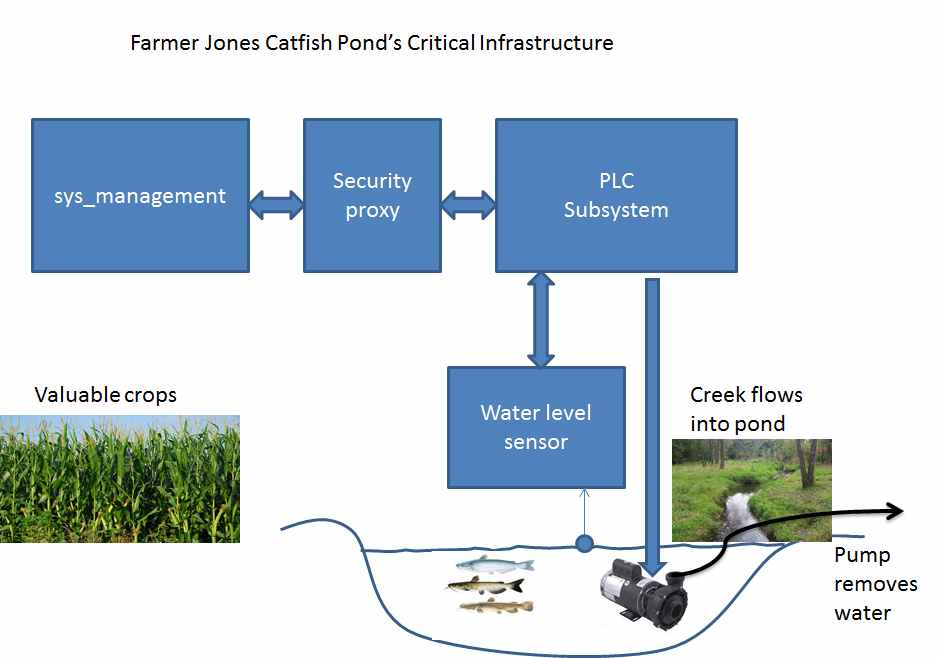
\includegraphics [width=0.8\textwidth,natwidth=621,natheight=403]{plc.jpg}
\end{center}
\end{figure}

You will interact with the sys\_management system to load a program and configuration data
into the PLC.  You will also use the sys\_management system to check the status of the PLC
and to query which program and configuration data the PLC is running. 
You will not have direct access to the PLC subsystem, though you can
interact with it via the sys\_management computer.

A "Security Proxy" sits between the sys\_management computer and the PLC.  The vendor promised
that this will prevent attacks on the PLC.  You can draw your own conclusions about that claim
You will interact with the Security Proxy in an attempt to make it useful.  But first, start the lab
as noted below (if you have not already done so).

\section {Performing the lab}
The lab is started from the Labtainer working
directory on your Docker-enabled host, e.g., a Linux VM.
From there, issue the command:
\begin{verbatim}
    ./labtainer plc
\end{verbatim}
\noindent The resulting virtual terminals will include: 
\begin{itemize}
\item A display of the status of the fish pond level, titled "Physical\_World".
\item A bash shell on the sys\_management computer.
\item A bash shell on the Security Proxy, titled "ubuntu@proxy".
\item A display of the Security Proxy log file titled "PROXY\_LOG".
\end{itemize}
NOTE: When the lab starts, observe the status window. The PLC is initially
disabled, and thus the pump does not run and the water rises.  
You can initialize the PLC from the sys\_management window using:
\begin{verbatim}
   ./manage_plc.py load plc config.txt
\end{verbatim}

\noindent The "plc" parameter is the name of the plc program file in your home directory.
The "config.txt" is a configuration file in your home directory.  This operation
will initialize the PLC, leading to the pump to run.

The configuration file directs the PLC to keep the pond level between 20 and 30 feet.
Just watch what happens over the course of about a minute.

After you've watched the status window for a full cycle of disaster, 
poke around a bit.  

\renewcommand\thesubsubsection{}
\subsubsection{Hints:}
\begin{itemize}
\item Use "stoplab plc" and "./labtainer plc" from your Linux host to stop and restart the lab -- this is the
best way to restart the lab or reset the PLC if it becomes corrupt.  Any files saved on the components will be preserved.
\item The manage\_plc.py tool lets your retrieve the code/data from the PLC.  Are those the files you loaded?
\item The sys\_management computer includes the openssl utility that you used in the onewayhash lab, might that
help determine if the files are the same?
\item Could the Security Proxy be modified to avoid sending bad files to the PLC?
\end{itemize}
NOTE: The solution must use the manage\_plc.py as-is. Modifying the code will void the warranty offered by the PLC system vendor!

\section {Tasks}
Alter the proxy.py program on the Security Proxy computer to prevent exploitation of the PLC.
You are not expected to make changes to the sys\_management system, though you are free to explore it.
However, credit will only be given if changes to the proxy.py mitigate the attack.
\end{document}


